% ------------------------------------------------------------------
\renewcommand{\thisweek}{MATH327 Week 10}
\renewcommand{\moddate}{Last modified 30 Apr.~2021}
\setcounter{section}{10}
\setcounter{subsection}{0}
\phantomsection
\addcontentsline{toc}{section}{Week 10: Interacting systems}
\section*{Week 10: Interacting systems}
\subsection{From non-interacting spins to the Ising model}
So far in this module we have considered `ideal' systems whose constituent objects do not interact with each other.
While we have seen that excellent mathematical models for real physical systems (such as stars and the cosmic microwave background) can be obtained despite this approximation of non-interacting particles, there are important statistical physics phenomena that cannot be captured by this approach.

An important class of examples, which we will investigate this week, are \textbf{phase transitions}, where interactions allow the same particles to produce extremely different large-scale behaviours, depending on control parameters such as the temperature or pressure.
An everyday example is the transition of H$_2$O molecules from liquid water to solid ice as the temperature decreases.
As the temperature of the universe itself decreased during the first few micro-seconds following the big bang, elementary particles transitioned from a so-called quark--gluon plasma to the protons and neutrons we are made out of today.
An intermediate example illustrated in the figure below (\href{https://doi.org/10.1063/PT.3.4384}{source}) involves two layers of graphene at a low temperature $T \approx 1.7$~K.
If these two layers are rotated with respect to each other by a small ``magic angle'' $\theta \approx 1.1^{\circ}$, the system transitions from being an electrical insulator to being a superconductor.

\begin{center}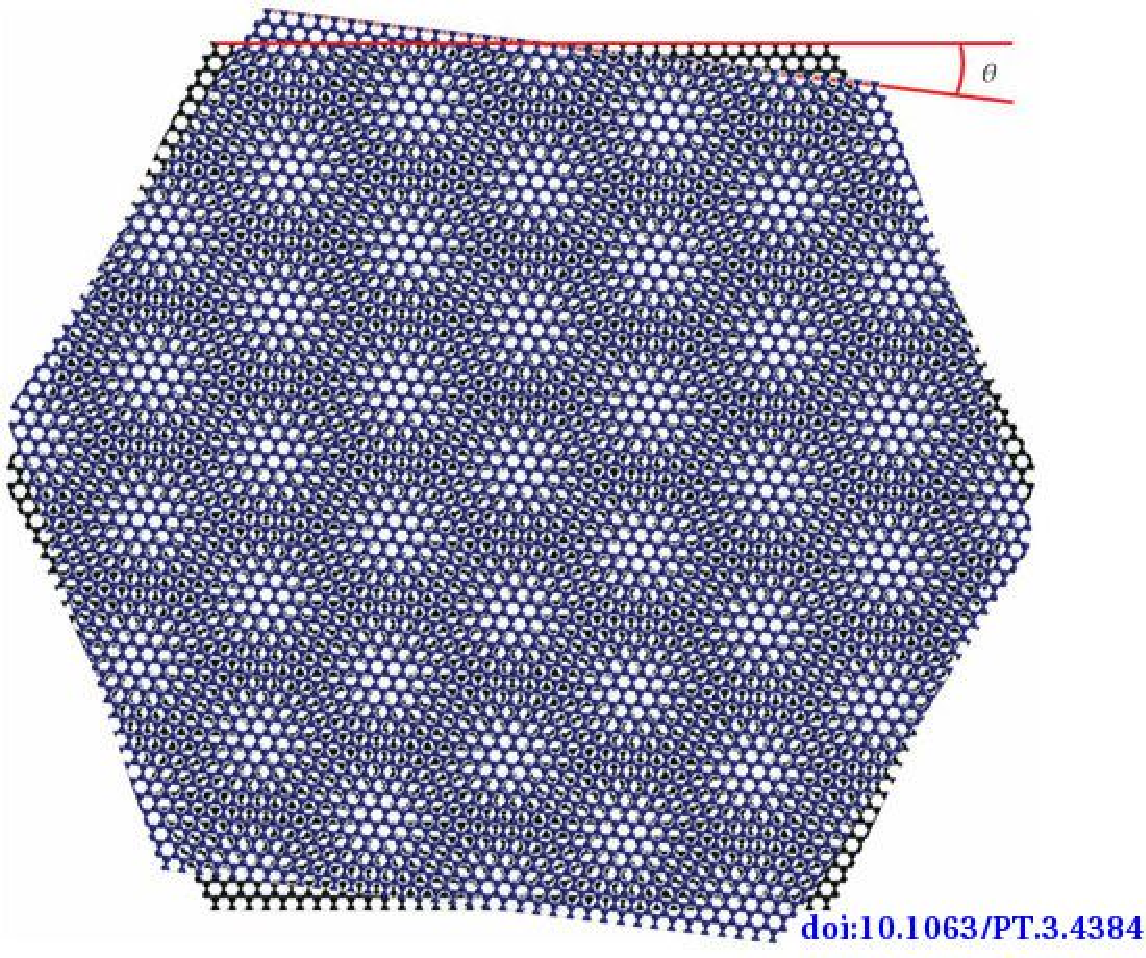
\includegraphics[width=0.5\textwidth]{figs/week10_graphene.pdf}\end{center}

We will introduce interactions and explore their effects using simple spin systems of the sort we previously analyzed in some depth during weeks $2$ and $3$.
In the non-interacting case we previously considered, the internal energy of the system (\eq{eq:spin_energy}) is
\begin{equation*}
  E = H \sum_{n = 1}^N s_n \qquad \mbox{(non-interacting)},
\end{equation*}
where $H > 0$ is the constant strength of an external magnetic field and the orientation of the $n$th spin, $s_n$, takes one of only two possible values: $s_n = 1$ if the spin is aligned anti-parallel to the field and $s_n = -1$ if the spin is aligned parallel to the field.
The ground state of the system features all $N$ spins aligned parallel to the magnetic field, with minimal energy $E_0 = -NH$.
This week we will only consider systems of distinguishable spins, which can be labeled by their fixed position in a $d$-dimensional simple cubic \textbf{lattice} like that shown below for $d = 2$ dimensions.
The $d = 1$ case of a one-dimensional lattice is precisely the system of spins arranged in a line that we analyzed in \secref{sec:spin_chain}.

\begin{center}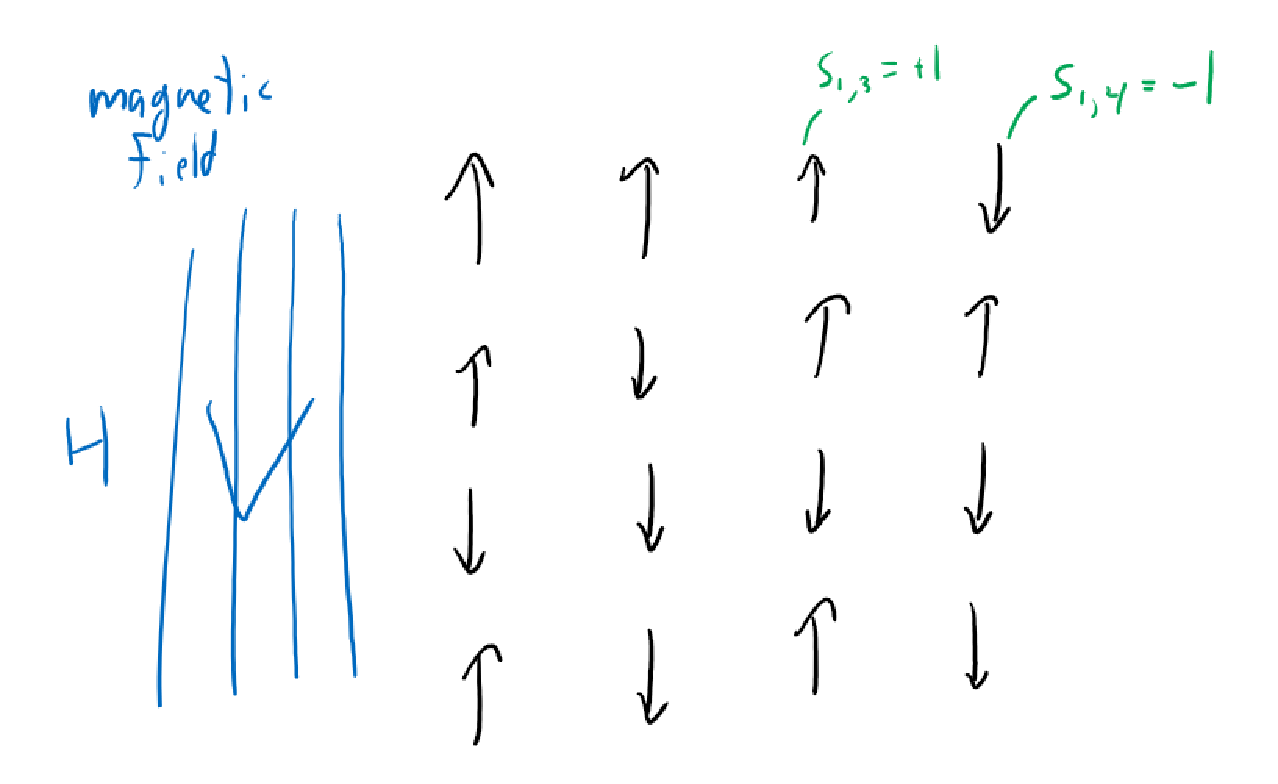
\includegraphics[width=0.8\textwidth]{figs/week10_spins.pdf}\end{center}

We can see that the total internal energy of the non-interacting system can easily be written as a sum over energies for each individual spin,
\begin{align*}
  E_n & = H s_n &
  E & = \sum_{n = 1}^N E_n \qquad \mbox{(non-interacting)}.
\end{align*}
This is a generic feature of non-interacting systems, and an aspect of the \textbf{factorization} that enormously simplifies calculations by causing the $N$-particle partition function (\eq{eq:spin_part_func}) to take the form of a product of $N$ identical terms, $Z = \left[2\cosh\left(\be H\right)\right]^N = Z_1^N$.
However, a stronger condition needs to be satisfied in order for such factorization to be guaranteed, which rigorously defines what it means for a system to be non-interacting.

\begin{shaded}
  Let $\De E_i$ be the change in the system's internal energy caused by changing its $i$th degree of freedom.
  Then the system is defined to be \textbf{non-interacting} if and only if $\De E_i$ is independent of all other degrees of freedom $k \ne i$.
\end{shaded}

For our system of $N$ distinguishable spins, the only possible change we can make to a degree of freedom is to negate it, $s_i \to -s_i$, which corresponds to flipping its alignment relative to the external magnetic field.
This spin flip causes the total energy to change,
\begin{equation*}
  E = H \sum_{n = 1}^N s_n = H\left(s_i + \sum_{k \ne i} s_k + \right) \quad \lra \quad H\left(-s_i + \sum_{k \ne i} s_k + \right),
\end{equation*}
corresponding to $\De E_i = -2H s_i$, which is indeed independent of all spins $s_k$ with $k \ne i$.
This simple check confirms that our definition works for the non-interacting spin system under consideration.

Now let's convert this setup into a system of interacting spins by adding the simplest possible two-spin contribution to its energy:
\begin{equation}
  \label{eq:Ising_energy}
  E = -\sum_{(ij)} s_i s_j + H \sum_{n = 1}^N s_n.
\end{equation}
The first sum runs over all pairs of nearest-neighbour spins in the lattice, denoted $(ij)$.
What is the change in energy $\De E_i$ from \eq{eq:Ising_energy} upon negating $s_i \to -s_i$?
Does this indicate an interacting or non-interacting system?
\begin{mdframed}
  \ \\[100 pt]
\end{mdframed}
The pictures below illustrate nearest-neighbour pairs for simple cubic lattices in $d = 2$ and $3$ dimensions, while also introducing some additional lattice terminology.

\begin{center}
  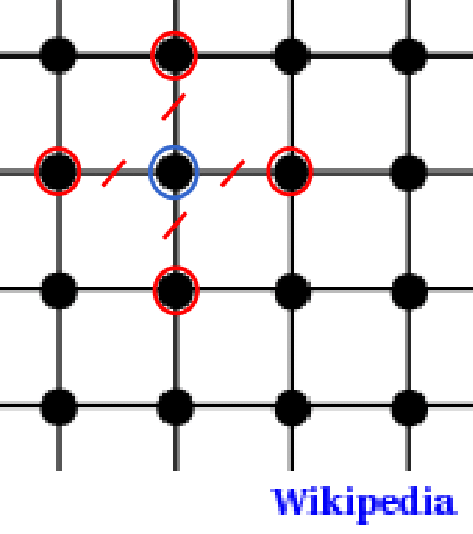
\includegraphics[height=0.4\textwidth]{figs/week10_lattice_2d.pdf}\hfill
  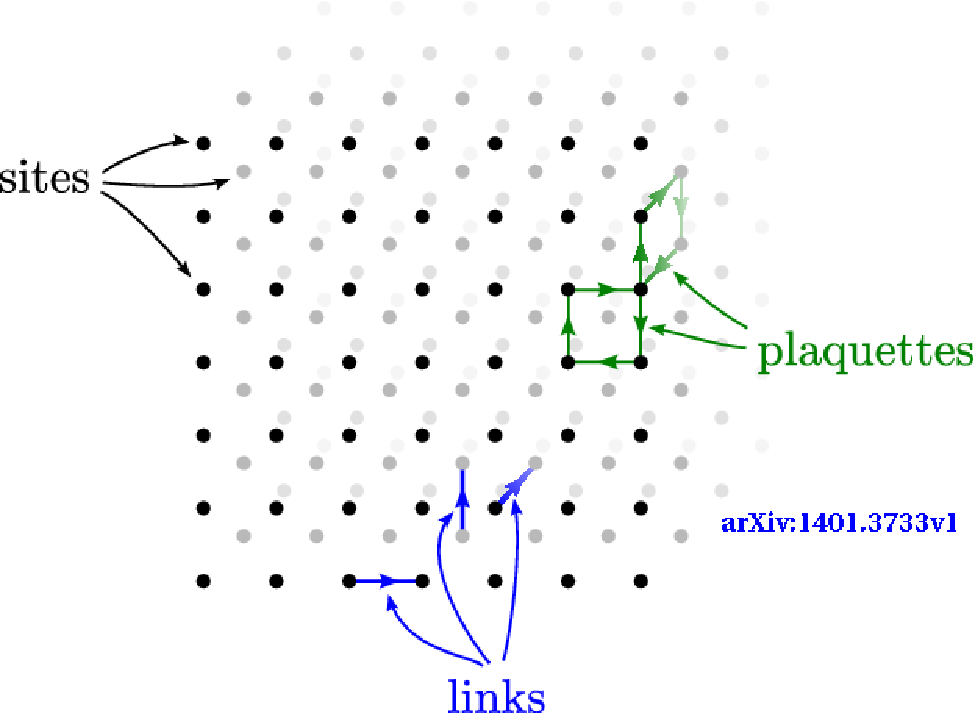
\includegraphics[height=0.4\textwidth]{figs/week10_lattice_3d.pdf}
\end{center}

Instead of drawing up- and down-pointing arrows, these pictures identify the spins with \textit{sites} in the lattice represented as points (or larger filled circles).
In simple cubic lattices, all sites are positioned in a regular grid, separated by a constant distance along each basis vector.
In between nearest-neighbour sites, we can draw \textit{links} as solid lines.
The picture of a two-dimensional lattice on the left highlights the four links (with red hatch marks) that correspond to the four nearest neighbours (circled in red) of a particular site (circled in blue).
While we can only have physical lattices with $d = 1$, $2$ or $3$ in nature, the mathematical construction works just as well for any integer $d \geq 1$.
For $d \geq 2$, an elementary unit of surface area is called a \textit{plaquettes}, while for $d \geq 3$ the elementary unit of volume is called a \textit{cube}.

Computing the energy in \eq{eq:Ising_energy} requires determining all of the nearest-neighbour pairs to be summed in the first term, which is equivalent to all of the links in the lattice, $\ell = (ij)$.
The only potential complication to this task is the need to consider what happens at the edges of the (finite) lattice.
We can avoid this complication by imposing \textbf{periodic boundary conditions}, which add an extra link between each site on the left edge of the lattice and a corresponding site on the right edge (and similarly in all other dimensions).
This is illustrated below for the simple one-dimensional lattice, which has been drawn as a circle to emphasize that all $N$ sites remain separated by a constant distance.
In higher dimensions, periodic boundary conditions produce flat (zero-curvature) $d$-dimensional tori that preserve the simple cubic lattice structure.

\begin{center}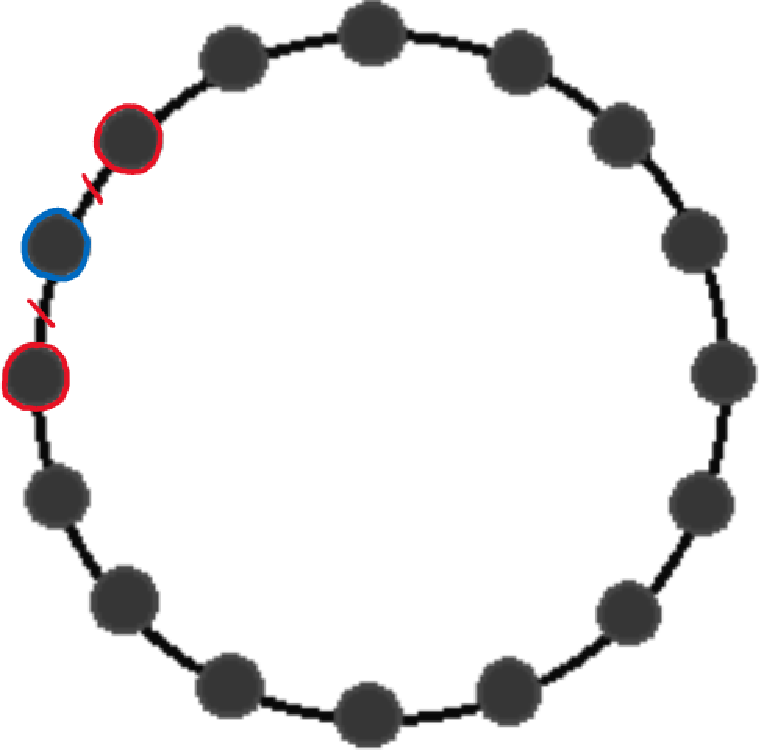
\includegraphics[width=0.45\textwidth]{figs/week10_lattice_1d.pdf}\end{center}

With periodic boundary conditions, we can easily see that the $N$-site one-dimensional lattice drawn above has $N$ links.
Each site has two links connecting it to its two nearest neighbours, and each of those links is shared between two sites, so that $\#\ell = 2N / 2 = N$.
Looking back to the two-dimensional lattice drawn farther above, the four links per site produce $\#\ell = 4N / 2 = 2N$.
How many terms are there in the sum $\sum_{(ij)}$ in \eq{eq:Ising_energy} for $N$-site lattices with periodic boundary conditions in $d$ dimensions?
\begin{mdframed}
  \ \\[50 pt]
\end{mdframed}

The energy in \eq{eq:Ising_energy}, with nearest-neighbour spins specified by the underlying simple cubic lattice structure, defines a famous system known as the $d$-dimensional \textbf{Ising model}.
Since the 1960s, the Ising model has been the basis of thousands of scientific studies analyzing everything from ferromagnetism to neural networks to urban segregation.\footnote{For a brief summary, see Charlie Wood, ``\href{https://www.quantamagazine.org/the-cartoon-picture-of-magnets-that-has-transformed-science-20200624/}{The Cartoon Picture of Magnets That Has Transformed Science}'', \textit{Quanta Magazine}, 24 July 2020.}
The model was proposed in 1920 by \href{https://en.wikipedia.org/wiki/Wilhelm_Lenz}{Wilhelm Lenz}, whose PhD student \href{https://en.wikipedia.org/wiki/Ernst_Ising}{Ernst Ising} solved the one-dimensional system as a research project in 1924.
Exactly solving the two-dimensional case (with $H = 0$) took another twenty years, culminating in renowned work by \href{https://en.wikipedia.org/wiki/Lars_Onsager}{Lars Onsager} in 1944.
The three-dimensional Ising model remains an open mathematical question, with no known exact solution.

In this context, `solving' the Ising model means deriving a closed-form expression for its canonical partition function,
\begin{equation*}
  Z(\be, N, H) = \sum_{\left\{s_n\right\}} \exp\left[-\be E(s_n)\right] = \sum_{\left\{s_i\right\}} \exp\left[\be\sum_{(ij)} s_i s_j - \be H \sum_n s_n\right].
\end{equation*}
As in \secref{sec:spin_info}, the partition function sums over all possible spin configurations $\left\{s_n\right\}$, which amounts to a sum of $2^N$ exponential factors for $N$ spins, with $\cO(N)$ terms within each exponential.
Now that the system is interacting, the partition function can no longer be factorized into $N$ identical two-term factors, making it extremely difficult to evaluate.
This is why there is no known exact solution to the three-dimensional Ising model, and it also makes `brute-force' numerical computations impractical.
Even for a system of $N = 1023$ spins (tiny compared to Avogadro's number $\sim 10^{23}$) there would be roughly $2^{1023} \sim 10^{310}$ terms in the partition function, far beyond the capabilities of existing or foreseeable supercomputers.
If we attempt `brute-force' numerical computation of every term in the partition function, even for a system of $N = 1023$ spins we would need to evaluate 
% ------------------------------------------------------------------



% ------------------------------------------------------------------
\subsection{Ising model phases and phase transition}
Similarly to how we analyzed non-interacting spin systems in \secref{sec:spin_info}, we can simplify the Ising model by considering its behaviour in the limits of high and low temperatures.


\TODO{Being written...}
% ------------------------------------------------------------------



% ------------------------------------------------------------------
\newpage
\subsection{The mean-field approximation}

\TODO{Being written...}
% ------------------------------------------------------------------



% ------------------------------------------------------------------
\newpage
\subsection{\TODO{Universality...}}
% TODO: Wilson, Kadanoff...

\TODO{Being written...}
% ------------------------------------------------------------------
